\documentclass[a4paper]{article}

\usepackage[utf8]{inputenc}
\usepackage[ngerman]{babel}
\usepackage[babel,german=quotes]{csquotes}
\usepackage[backend=biber,maxnames=99,language=german,style=alphabetic,sortcites=true]{biblatex}
\usepackage{a4wide}
\usepackage{graphicx}
\usepackage{amscd}
\usepackage{amssymb}
\usepackage{amsmath}
\usepackage{bibgerm}
\usepackage[hidelinks]{hyperref} %add [hidelinks] to hide link boxes
\usepackage{gensymb}
\usepackage[section]{placeins}
\usepackage[export]{adjustbox}
\usepackage{bm}
\usepackage{centernot}

\usepackage{xcolor}
\usepackage{textcomp}
\usepackage{listings}

\usepackage{ifthen}
\usepackage{eurosym}			%add euro symbol
%\usepackage{showframe}			% show all kind of frames that latex uses
%\usepackage{refcheck}			% checks for wrong refs

\newcommand{\qq}[1]{\glqq #1\grqq{}}

\newcommand{\vcDash}[1]{\ifthenelse{\equal{#1}{-}}{\text{-}}{#1}}
\newcommand{\vc}[3]{$(\vcDash{#1}, \vcDash{#2}, \vcDash{#3})$}


\hbadness=10000
\clubpenalty = 10000 % schliesst Schusterjungen aus
\widowpenalty = 10000 % schliesst Hurenkinder aus

\lstset{
	 literate={ö}{{\"o}}1 	%Replaces "oe","ae" usw. with \o to use "Umlaute" in listings
           {ä}{{\"a}}1
           {ü}{{\"u}}1
	{ß}{{\ss}}1
	{Ö}{{\"O}}1
	{Ä}{{\"A}}1
           {Ü}{{\"U}}1
	{ß}{{\ss}}1,
  	breaklines=true,                		% sets automatic line breaking
	moredelim=[is][\bfseries]{[*}{*]},   	% enable bold style with "[*text*]" in lstlisting
	columns=flexible
}

	\definecolor{light-gray}{gray}{0.95}

\lstdefinelanguage{sharpc}{
	basicstyle=\fontsize{10pt}{12pt}\ttfamily,
	language=[Sharp]C, 
	rulecolor=\color{blue!80!black},
	morekeywords={,async, await, var,where, }
	tabsize=3
}

\lstset{language=sharpc,
	showspaces=false,
	showtabs=false,
	tabsize=4,
	breaklines=true,
	keepspaces=true,      
	numbers=left,
	numberstyle=\scriptsize,
	stepnumber=1,
	numbersep=8pt,
	showstringspaces=false,
	breakatwhitespace=true,
	commentstyle=\color{green},
	keywordstyle=\color{blue},
	stringstyle=\color{red},
	basicstyle=\ttfamily,
	backgroundcolor=\color{light-gray},
	%  moredelim=[il][\textcolor{pgrey}]{$$},
	%  moredelim=[is][\textcolor{pgrey}]{\%\%}{\%\%}
}

\graphicspath{{./img/}}

%%%
%%% Style-Definition des Literaturverzeichnis
%%%
%%

%\bibliographystyle{is-alpha}
%\bibliographystyle{geralpha}
\bibliography{hausarbeit}
\addbibresource{hausarbeit.bib} 
 
 
%%\setlength{\parindent}{0pt} %kein Einzug beim Absatzbegin
\setlength{\parskip}\medskipamount %Abstand zwischen 2 Abs�tzen
\setcounter{tocdepth}{4} 
\setcounter{secnumdepth}{4}

\author{Markus Bullman, Julius Hackel}
\title{Hausarbeit \\ Ausgewählte Probleme der Verteilten Systeme \\ Vector Clock}
\begin{document}

\maketitle
\clearpage

\noindent Folgende Abschnitte wurden von den entsprechenden Personen verfasst:
\begin{tabbing}
    Markus Bullmann:~~~~~~~~~ \= Kapitel 1, 2 und 4 \\
    Julius Hackel:        \> Kapitel 3, 5 und 6 \\
\end{tabbing}
\begin{center}\noindent\rule{10cm}{0.4pt}\end{center} ~\\
Hiermit versichere ich, dass ich die vorgelegte Arbeit selbstständig verfasst und noch nicht
anderweitig zu Prüfungszwecken vorgelegt habe. Alle benutzten Quellen und Hilfsmittel sind
angegeben, wörtliche und sinngemäße Zitate wurden als solche gekennzeichnet.\\[15mm]
Würzburg, den\\[20mm]

\begin{center}(Markus Bullmann) \hspace{60mm} (Julius Hackel)\end{center}

\clearpage

\tableofcontents
\clearpage

\section{Einleitung}
\subsection{Motivation}
\subsection{Zielsetzung}
\subsection{Aufbau}

\cleardoublepage
\section{Arten von Uhren}
In diesem Kapitel werden unterschiedliche Uhrtypen vorgestellt.
\subsection{Physikalische Uhren}
\subsection{Lamport Uhren}
\subsection{Vektor Uhren}
\subsection{Interval Tree Uhren}
\cleardoublepage
\section{Funktionsweise von Vektoruhren}
\subsection{Prinzipielle Funktionsweise}

Wie bereits beschrieben wurde, bilden Vektoruhren eine Erweiterung der Lamportuhr. Dabei wird pro Node im System ein Integer als Zähler für den Node in der Vektoruhr gespeichert. Im Allgemeinen werden durch eine Vektoruhr Zeitstempel mit Events im System assoziiert \cite{Baldoni:2002:FDC:1435723.1437765}[S. 3].

Jeder Node im System besitzt seine eigene Vektoruhr in der Form eines Vektors $VC_i[1...n]$, wobei alle Elemente der Uhr mit $0$ initialisiert werden. Die Uhr eines Nodes wird wie folgt verwaltet und aktualisiert:

\begin{itemize}
	\item[R1]Jedes mal, wenn ein Node $P_i$ ein Event auslöst, muss dieser seine Vektoruhr für den Eintrag $VC_i$ um Eins hochzählen, es gilt  $VC_i[i] := VC_i[i] + 1$. Dadurch verdeutlicht der Node, dass er etwas getan hat und signalisiert dies den anderen Nodes durch aktualisieren seiner Vektoruhr 
	\item[R2]Sendet ein Node $P_i$ eine Nachricht $m$, so hängt er seine aktuelle Vektoruhr $VC_i$ an die zu sendende Nachricht an. Auf diese Weise gelangt die Uhr zu dem Empfänger der Nachricht.
	\item[R3]Empfängt ein Node $P_i$ eine Nachricht, so muss er seine Vektoruhr aktualisieren. Dabei geht er wie folgt vor: $VC_i = \max(VC_i, m.VC)$. Dies bedeutet, dass der Node für jedes Element seiner Vektoruhr überprüft ob der Wert in der Uhr der Nachricht größer als der eigene ist. Sollte dies der Fall sein, wird der eigene Wert an dieser Stelle mit dem Wert aus der anderen Uhr überschrieben.\label{R3}
\end{itemize} \cite{Baldoni:2002:FDC:1435723.1437765}[S. 4]

Die Werte innerhalb einer Vektoruhr $VC_i$ haben eine besondere Bedeutung für den Node $P_i$. $VC_i[i]$ gibt die Anzahl an Events an, welche $P_i$ zu dem Zeitpunkt des Betrachtens verarbeitet hat. Die anderen Werte der Uhr ($VC_i[j]$ mit $j \neq i$) zeigen an, dass alle Events welche durch den Node $P_j$ verarbeitet wurden, sich kausal betrachtet in der Vergangenheit von $P_i$ befinden. Sie geben sozusagen an, was Node $P_i$ über die Zeiten der anderen Nodes weiß, diese Information kann sich zu dem Zeitpunkt jedoch bereits von den tatsächlichen Zeiten unterscheiden. Da jeder Node lediglich seinen Zähler in der Vektoruhr erhöhen darf, hat dieser Node zu jedem Zeitpunkt den aktuellsten Stand seiner lokalen Zeit. \cite{SINGHAL199247}[S. 48]

\subsubsection{Vergleich von Vektoruhren untereinander}
Eine Besonderheit der Vektoruhren besteht im Vergleich von Uhren untereinander. Dies wird notwendig, sobald ein Node eine Nachricht erhält und diese verarbeiten muss. Wie in Bedingung R3 unter \ref{R3} - \nameref{R3} zu sehen, muss der Node seine Uhr entsprechen der mitgeschickten Vektoruhr der Nachricht aktualisieren. Der Vergleich zwischen der eigenen und der empfangenen Uhr muss dann auf Anwendungsebene geschehen, denn dort wird entschieden was mit der angekommenen Nachricht geschieht.

Für zwei zu vergleichende Uhren $VC_1$ und $VC_2$ gibt es folgenden Beziehungen:

\begin{eqnarray}
&VC_1 \leq VC_2& \text{ wenn } \forall i : VC_1[i] \leq VC_2[i] \\
	&VC_1 < VC_2& \text{ wenn } VC_1 \leq VC_2 \text{ \& } VC_1 \neq VC_2 \\
	&VC_1 \mid \mid VC_2& \text{ wenn } !(VC_1 < VC_2) \text{ \& } !(VC_2 < VC_1)
\end{eqnarray}
\cite{Mattern88virtualtime}[S. 127, Definition 4]

Fall (1) bedeutet, dass eine Uhr $VC_1$ kleiner oder gleich $VC_2$ ist, wenn jedes Element von $VC_1$ kleiner oder gleich dem entsprechenden Element in $VC_2$ ist. Der zweite Fall (2) liegt vor, wenn Fall (1) zutrifft und zusätzlich kein Element in $VC_1$ gleich dem entsprechenden Element in $VC_2$ ist. 
Der letzte Fall (3) ist ein Besonderer Fall. Dieser trifft ein wenn nicht entschieden werden kann, welche Uhr neuer oder älter beziehungsweise nach der obigen Definition größer oder kleiner ist als die andere. Die entsprechenden Nachrichten wurden sozusagen gleichzeitig abgeschickt. Dieser im Englischen als Concurrent bezeichnete Fall stellt ein großes Problem für Systeme dar, die Vektoruhren für die zeitliche Synchronisation der Kommunikation nutzen. Auf diesen Sonderfall wird im nächsten Kapitel genauer eingegangen.
\subsubsection{Beispiel einer Kommunikation}
Um die Funktionsweise von Vektoruhren genauer zu beschreiben, wird nun anhand eines einfachen Beispieles die Kommunikation in einem System mit drei Nodes sowie die Verarbeitung der Vektoruhren eines jeden Nodes gezeigt.

TODO: Beispiel schrittweise zeigen und Uhren beschreiben

\subsection{Umsetzung in C\#}
Für die Umsetzung dieses Themas wurde C\# als Programmiersprache ausgewählt. Damit die zeitliche Synchronisation mittels Vektoruhren möglichst realitätsnah simuliert werden kann, wurden drei virtuelle Maschinen mit dem Betriebssystem Windows 8.1 aufgesetzt. Diese befinden sich im Hochschulnetzwerk und können per Remote Desktop bedient werden.

Die Implementierung wurde in zwei unabhängige Programmteile aufgeteilt. Diese sind ein Commander sowie Nodes. 

TODO: Abbildung des Gesamtsystemes (Commander + 3 Nodes)

Der Commander stellt sozusagen eine übergeordnete Kommandozentrale dar, welche die Kommunikation der Nodes untereinander durch gewisse Steuerbefehle koordiniert. Er besitzt eine grafische Oberfläche, welche mittels WPF erstellt wurde.

\begin{figure}[ht]
	\centering
	\includegraphics[width=10cm]{commanderWindow.png}
	\caption[Commander Window]{Abbildung des Commanderfensters, welcher dazu dient, die Kommunikation zwischen den Nodes durch Steuerbefehle zu koordinieren}}
	\label{figure:commanderWindow}
\end{figure}
\FloatBarrier

Ein Node stellt einen Knoten in dem simulierten System dar. In diesem werden Events ausgeführt und Vektoruhren verarbeitet. Jeder Node besitzt seine eigene, lokale Vektoruhr. Bei einem Node handelt es sich um ein Kommandozeilenprogramm, welches auf einer VM läuft und ständig auf Nachrichten wartet. Damit der Ablauf der Kommunikation besser nachvollzogen werden kann, gibt ein Node bei jedem Event die Details der Nachricht sowie seiner Vektoruhr aus. Zusätzlich sendet er dabei eine Antwort an den Commander mit der Nachricht, welche er erhalten hat und seiner aktuellen lokalen Uhr. Der Commander gibt diese empfangene Antwort in einem Textfenster aus.

\begin{figure}[ht]
	\centering
	\includegraphics[width=10cm]{nodeWindow.png}
	\caption[Node Window]{Abbildung des Nodefensters. Zwischen den Nodes findet die eigentlichen Kommunikation statt.}
\label{figure:nodeWindow}
\end{figure}
\FloatBarrier

Die Kommunikation zwischen dem Commander und den Nodes wurde mittels UDP realisiert. Die Entscheidung viel auf UDP, da sich dadurch unnötiger Overhead und Programmieraufwand vermeiden lässt, welcher beispielsweise bei TCP angefallen wäre. Der Aufbau einer Nachricht ist in Abbildung \ref{Nachricht} dargestellt. Beim Absenden der Nachricht, egal ob im Commander oder in den Nodes, wird diese serialisiert und per UPD versendet. Im Empfangsfall muss der empfangene Datenstrom wieder deserialisiert und in eine Nachricht umgewandelt werden. 

\cleardoublepage
\section{Schwierigkeiten von Vektoruhren}
\label{cap:problemeVC}
\subsection{Effizienten Speicherung von Vektoruhren}
% Paper: Concerning the size of clocks 
%        Plausible Clocks Constant Size Logical Clocks for Distributed Systems
Vektoruhren sind eine relativ einfache und effektive Lösung kausale Ordnung in einem verteilten System herzustellen.
Ihre Definition beherbergt jedoch ihren größten Nachteil.
Die Größe einer Uhr ist nicht konstant.
Für ein verteiltes System mit $n$ Prozessen benötigt eine Vektoruhr $n$ Komponenten i.d.R. Integer-Zahlen.
Die Folge ist, dass für ein großes verteiltes System alle Vektoruhren einen entsprechend hohen Speicherbedarf haben.
Dies wirkt sich zum einen negativ auf den Speicherverbrauch der einzelnen Prozesse aus, da je nach Implementierung mehrere Uhren gespeichert werden müssen.
Außerdem fügen die großen Vektoruhren einen Overhead zu den Nachrichten hinzu und belasten somit den Übertragungsweg.
Offensichtlich ist die Länge der Vektoruhr direkt proportional zur Anzahl der Prozesse.
Somit skalieren Vektoruhren schlecht \cite{torres1999plausible}.

Charron-Bost \cite{charron1990concerning} hat bewiesen, dass es innerhalb eines Systems bestehend aus $n$ Nodes immer eine mögliche Kombination an Ereignissen geben kann, bei der die Kausalität ausschließlich mit Vektoruhren der Länge $n$ erfasst werden kann.
Von daher müssen für alle theoretisch vorkommenden Prozesse innerhalb des Systems eine Komponente in der Uhr reserviert werden.
Dies beinhaltet alle aktuellen Prozesse und auch zukünftige Prozesse die möglicherweise ausgeführt werden könnten.
Es ist natürlich schwer im voraus zu entscheiden wie viele Prozesse potentiell ausgeführt werden und ist daher im Allgemeinen nur bei statischen Systemen gegeben, bei denen also  bei denen also die Anzahl der Prozesse konstant ist.
Daher muss theoretisch eine Vektoruhr mit einer statischen Länge von $n$ verwendet werden.
Im Folgenden werden verschiedene Verfahren vorgestellt um die Länge von Vektoruhren zu reduzieren.

Ein pragmatisches Vorgehen um die Länge einer Vektoruhr in einer annehmbarer Größe zu halten wurde von Amazon in ihrer Dynamo Datenbank \cite{decandia2007dynamo} verfolgt.
Hierbei wird die Länge durch folgendes Kürzungsschema reduziert:
Zu jeder Komponente in der Vektoruhr wird neben dem Zähler noch die Prozess ID und ein Zeitstempel gehalten.
Der Zeitstempel gibt den Zeitpunkt an, zudem der entsprechende Prozess zuletzt den Datensatz aktualisierte.
Erreicht die Länge der Vektoruhr einen bestimmten Schwellwert, werden die Komponenten mit den ältesten Zeitstempel aus der Uhr entfernt.
Dieses Verwerfen von Daten kann dazu führen, dass in gewissen Situationen die Kausalität nicht mehr komplett hergestellt werden kann.
Nach eigenen Angaben von \etal{DeCandia} \cite{decandia2007dynamo} trat dieses Problem im Produktiveinsatz jedoch nicht auf und wurde daher nicht weiter analysiert.

\etal{Singhal} \cite{singhal1992efficient} stellten ein einfaches Verfahren vor um den Overhead bei der Nachrichtenübertragung im Durchschnitt zu verringern.
Ihre Technik basiert auf der empirischen Beobachtung, dass nur wenige Prozesse häufig miteinander kommunizieren.
Außerdem ist es wahrscheinlich, dass zwischen zwei aufeinanderfolgend Sende-Ereignisse von Prozess $P_i$ zu $P_j$ nur wenige Komponenten der Vektoruhr sich ändern.
In diesem Fall ist es unnötig die komplette Uhr mit jeder ausgehenden Nachricht von $P_i$ zu $P_j$ zu übertragen.
Es ist ausreichend nur die Komponenten zu übertragen die sich geändert haben.
Konkret kann bei einer gegeben Uhr $VC$ für jede geänderte Komponenten ein Tupel aus $(a, VC[a])$ übertragen werden, wobei $a$ dem Index des Prozess innerhalb der Uhr entspricht.
Werden Vektoruhren nach dieser Technik übertragen kann die zu übertragene Datenmenge reduziert werden.
Dabei wird jedoch der lokale Speicherbedarf eines Prozesses erhöht, da dieser zusätzlich speichern muss welche Werte zuletzt zu welchen Prozess geschickt wurden.
Anhand den gespeicherten Vektoren kann er die entsprechenden Tupel auswählen, die an eine Nachricht mit angehängt werden müssen.

\begin{figure}[ht]
    \centering
    \includegraphics[width=1\textwidth]{Singhal.png}
    \caption[Kommunikaiton nach Singhal]{Ablauf der Kommunikation dreier Prozesse nach dem Verfahren von \etal{Singhal}.}
    Quelle: Nachgezeichnet aus \cite{Baldoni:2002:FDC:1435723.1437765}
    \label{fig:singhal}
\end{figure}

Bisher wurde immer angenommen, dass die Anzahl der Prozesse innerhalb eines Systems konstant ist.
Dies ist jedoch selten der Fall, in der Regel werden Prozesse häufig gestartet und beendet.
Die Folge ist, dass bei einer naiven Implementierung der Vektoruhr für jeden jemals ausgeführten Prozess eine Komponente in der Uhr reserviert werden muss.
In dynamischen Systemen kann dies dazu führen, dass die Uhren schnell eine tragbare Größe überschreiten.
Es ist daher wünschenswert Vektoruhren für solche dynamische Systeme zu optimieren.

Fridge \cite{fidge1991logical} stellte ein Modell vor bei dem eine variable Anzahl an Prozess-IDs verwendet wird.
Hierbei müssen die Prozess-IDs innerhalb des Systems eindeutig sein.
Beim Start eines Prozesses wird ihm eine ID zugewiesen.
Die ID eines terminierten Prozesses wird jedoch nicht freigegeben.
Damit die IDs solcher Prozesse freigegeben werden können, müssen allen anderen Prozesse die Terminierung bekannt sein.
Ist dies nicht gegeben, darf die ID nicht aus der Vektoruhr entfernt werden.
Diese Art von Garbage Collection wird in \cite{richard1998efficient} verwendet.
Alle Verfahren dieser Art haben jedoch das Problem, dass IDs von terminierten Prozessen nicht wiederverwendet werden können und die Bereinigung der Uhr von terminierten Prozessen durch einen einzigen unerreichbaren Prozess bereits verhindert werden kann \cite{almeida2008treeclocks}.

% Hier würde Landes reinpassen

Wie gezeigt führt die Verwendung von globalen IDs zu neuen Problemen.
Es liegt somit nahe auf globale IDs gänzlich zu verzichten.
Aus dieser Überlegung heraus entwickelten \etal{Almeida} \cite{almeida2008treeclocks} eine Generalisierung von Vektoruhren.
Die sogenannten \qq{Interval Tree Clocks} sind für dynamische Systeme ausgelegt und kommen dabei ohne globale IDs aus, indem jeder Prozess selbständig neue IDs erzeugen, löschen oder wiederverwenden kann, ohne das dabei auf eine globale Kommunikation zurückgegriffen werden muss.
Durch teilen und zusammenfassen von Prozess IDs wachsen und schrumpfen die Zeitstempel entsprechend zu der Dynamik des Systems.
Der Platzbedarf der Zeitstempel skaliert somit mit der Anzahl der Prozesse und wächst nur moderat an \cite{almeida2008treeclocks}.

% \cite{almeida2008treeclocks}
% landes dynamic clock

Ein in der Praxis relevantes Problem ist die Handhabung von Integer Überlaufen der Zählern innerhalb der Uhr.
In der Theorie werden die natürlichen Zahlen als Menge der möglichen Zählerwerte angenommen und haben somit keine Beschränkung.
Bei der Implementierung einer Vektoruhr muss jedoch über die Darstellung der Vektorkomponenten entschieden werden.
In der Regel wird ein Integer Datentyp mit typischerweise 32 oder 64 Bit gewählt.
Dabei muss ein Kompromiss zwischen maximale Länge und Datenmenge die zu übertragen ist gefunden werden.
Wird das verteilte System lange genug ausgeführt oder treten hochfrequent Ereignisse auf, kann es durchaus passieren, dass die Bitgrenze des gewählten Datentyps erreicht ist und ein Overflow zur Folge ist.
Dabei springt der Zähler vom Maximalwert auf Null.
\etal{Yen} \cite{yen1997resetting} stellen hierzu ein Protokoll vor um die Uhren zurückzusetzen.
Wird dieses Schema implementiert kann bei manche Anwendungen darauf verzichtet werden die optimale Bitlänge der Vektorkomponenten zu bestimmen. Da lediglich ein geeigneter Auslöser für den Uhrenreset gefunden werden muss \cite{yen1997resetting}.
Ein allgemeingültiges Verfahren wurde von Baldoni \cite{baldoni1998positive} vorgestellt.

% cap:vectorclock
\subsection{Gleichzeitig abgesendete Nachrichten}
\label{lbl:consistency}
% Verteiltes System
% Replika
% Konsitenz 
consistency

% Strong
>
Causal
>
Eventual

Wie bereits in der Einführung erwähnt, existiert kein globaler Zustand in einem verteilten System.
Vielmehr wird die Vereinigung aller lokalen Zustände als globaler Zustand verstanden.
Voraussetzung hierzu ist, dass alle Prozesse zu einem gewissen Zeitpunkt den selben lokalen Zustand haben.

Konkret kann es sich bei einem globalen Zustand zum Beispiel um ein Datenfeld in einer verteilten Key-Value-Datenbank handeln.
Jedes Datenfeld kann durch einen eindeutigen Schlüssel aus der Datenbank ausgelesen werden.
Alle Prozesse halten eine Replikation dieser Schlüssel-Werte Paare.
Durch die Kopie hat sich die Identität der Entität nicht geändert, das heißt obwohl eine Kopie gemacht wurde, handelt es sich immer noch um das selbe Objekt.

Wird nun in einem Prozess dieses Datenfeld modifiziert, muss die Änderung allen anderen Prozessen bekannt gemacht werden, damit diese den neuen Wert annehmen können.
Solange die Prozesse nach einer Datenänderung unterschiedliche Werte haben, ist das System inkonsistent, da je nachdem an welchem Prozess die Entität abgefragt wird, ein abweichender Wert zurück gegeben werden kann.
Der Umgang mit Änderungen und der Tolerierung eines solchen Zeitfensters, indem das System inkonsistent ist, führt zu einer Klassifizierung nach Konsistenzmodelle.

Es existieren eine Vielzahl an unterschiedlichen Modelle, die auf einer Skala von schwach nach strikt geordnet werden können.
Bei strikter Konsistenz (engl. \qq{strong consistency}) sind alle Replika immer identisch. Dies wird erreicht indem jedes Replika in der selben Reihenfolge aktualisiert wird und die Aktualisierung atomar durchgeführt wird.

Bei der Entwicklung einer verteilten Applikation aufbauend auf einer verteilten Datenbank mit strikter Konsistenz treten, im Vergleich zu einer herkömmlichen Datenbank, keine zusätzliche Schwierigkeiten auf.
Durch die strikte Konsistenz können keine Dateninkonsistenzen auftreten, ähnlich einer herkömmlichen relationalen Datenbank.
Gleichzeitig ist sie aber das teuerste Modell in der Umsetzung, da ein großer Kommunikationsaufwand betrieben werden muss.

Schwache Konsistenz (engl. \qq{weak consistency}) fordert, dass jedes Replika zu irgendeinen Zeitpunkt alle Aktualisierungen erhalten wird, ohne Forderungen an der Reihenfolge zu stellen.
Ein Applikation kann sich daher kaum auf die verteilte Datenbank verlassen, da durch die schwache Konsistenz kaum Versprechen über die Aktualität der Daten gemacht wird.
So kann eine spätere Aktualisierung eine frühere überschreiben, wenn ihre Nachricht schneller zugestellt wurde als die konkurrierende Nachricht.

Zwischen schwacher und strikter Konsistenz kann die sogenannte eventual consistency eingeordnet werden.
Ähnlich zur schwachen Konsistenz werden hier keine Leseinkonsistenzen eliminiert, zwei direkt aufeinander folgende Leseoperationen könne zwei unterschiedliche Werte ausgeben.
Es wird jedoch garantiert, dass sich das System stabilisieren und zu einem bestimmten Zeitpunkt alle Replika den selben Wert haben werden.
Die Aktualisierungen können in einer anderen Reihenfolge von einem Prozess empfangen werden, als sie gesendet wurden.
Der Prozess muss jedoch in der Lage sein die Aktualisierungen zu ordnen um den endgültigen Wert ohne Datenverlust zu bestimmen.

Einige verteilte System fordern nur sehr schwache Konsistenzbedingungen.
So ist die eventual consistency ein häufig implementiertes Konsistenzmodell.
Ein Beispiel für eine verteilte Datenbank die nach eventual consistency arbeitet ist Dynamo von Amazon \cite{decandia2007dynamo}.
Hier wird zu Gunsten der Geschwindigkeit auf eine strenge Konsistenz verzichtet.

Amazon setzt in ihrer Dynamo Datenbank Vektoruhren ein, um die Aktualisierungen in ihrer korrekten Ordnungen anzuwenden, wie es von eventual consistency gefordert ist.
Hierzu erhält jedes Objekt seine eigne Vektoruhr und fungiert als Version des Objekts.
Wird ein Replika verändert, inkrementiert es die Vektoruhr des Datenfeldes und teilt alle anderen Replika die Werteänderung mit.
Erhält ein Replika eine Aktualisierung zu der eine vorhergehende Aktualisierung noch nicht bei dem zu verarbeiteten Prozess angekommen ist, muss diese aufgeschoben werden.
Durch die Vektoruhr kann in den meisten Fällen bestimmt werden, welche Schreiboperation zuvor durchgeführt wurde.
In \fig{fig:vecConcurrent} ist eine solche aufgeschobene Aktualisierung dargestellt.

\begin{figure}[ht]
    \centering
    \includegraphics[width=0.8\textwidth]{VektorConcurr.pdf}
    \caption[Aufheben von Nachrichten]{Grafische Darstellung zweier Konflikte. Zum einen muss eine Nachricht richtig eingeordnet werden, da sie überholt wurde und zum anderem wurden die Nachrichten zu $e_1$ und $e_2$ gleichzeitig verschickt.}
    \label{fig:vecConcurrent}
\end{figure} 

Es kann jedoch passieren, dass durch die Vektoruhr keine Reihenfolge zwischen zwei Aktualisierungen festgestellt werden konnte, nämlich genau dann wenn $e_1 \parallel e_2$ gilt.
Diese nebenläufige Schreiboperationen, also Operationen die noch nicht abgeschlossen sind bevor Neue ausgeführt werden, stellen ein Problem für die eventual consistency dar.
Um einen Datenverlust zu vermeiden muss entschieden werden, in welcher Reihenfolge die Schreiboperationen ausgeführt werden sollen.
Die Schwierigkeit besteht jedoch darin, dass die Vektoruhr keine Aussage hierzu treffen kann.
\fig{fig:vecConcurrent} zeigt zwei gleichzeitig aufgetretene Schreiboperationen $e_1$ und $e_3$.
Durch die Vektoruhren kann auf die Nebenläufigkeit $e_1 \parallel e_3$ getestet werden:
\begin{align*}
      VC_3(e_3)[1] & \leq VC_1(e_1)[1] & \wedge & & VC_1(e_1)[3] & \leq VC_3(e_3)[3] \\
         3         & \leq 4            & \wedge & & 0            & \leq 2
\end{align*}

Da es sich hierbei um eine wahre Aussage handelt gilt, dass $e_1$ und $e_2$ gleichzeitig aufgetreten sein müssen.
Nun muss entschieden werden wie mit so einer Situation umgegangen wird.
Da die Middelware, die in der Regel die Handhabung der Vektoruhr übernimmt, keinerlei Informationen über den Inhalt der Datenfelder oder generell über die kommunizierten Daten hat, kann sie nur den Konflikt an die Applikationsschicht melden und eine Auflösung des Konflikts anfordern.
Wie die Applikation endgültig den Konflikt löst ist stark anwendungsabhängig und unterscheidet sich von Fall zu Fall.
Eine einfache, jedoch mit Datenverlust behaftete Lösung ist es die letzte Schreiboperation zu übernehmen und die ältere zu verwerfen.

Die Amazon Datenbank unterscheidet generell zwischen syntaktische und schematische Konflikte.
Können die Operationen durch die Vektoruhren kausal geordnet werden, gilt der Konflikt als syntaktisch gelöst.
Ist dies nicht möglich muss er schematisch gelöst werden, also durch die Applikationsschicht.


\subsection{Aufheben alter Nachrichten}
% 1. Ereignisse müssen alle Prozesse mitgeteilt werden. Nachrichten müssen solange aufgehoben werden, bis alle die Nachricht erhalten haben. Anhand von Nachrichten der anderen Prozessen kann mit deren Vektorclock entschieden werden welche Nachrichten sie von einem selbst schon haben
% 2. Nachrichten müssen für eventual Consitiency aufgehoben werden. Daei kann es passieren, dass eine Nachricht rein kommt die bereits die alten Zustände enthält und somit die alten Nachrichten obsolete.
% 3. Matrix Clock 'fire and forget'
% http://stackoverflow.com/questions/21359184/what-do-matrix-clocks-solve-but-vector-clocks-cant
% Voraussetzung: eventual consistency
% Zeigen Ohne Matrix würde es nicht gehen
% Matrix Uhren ermöglichen GC
Anhand Vektoruhren kann entschieden werden, wann zwischengespeicherte Nachrichten gelöscht werden können.
Hierzu gibt es drei potentielle Situationen in denen, entschieden werden muss wann etwas sicher gelöscht werden kann.
Für die ersten Beiden können Vektoruhren angewendet werden und für die letzte muss eine Erweiterung von Vektoruhren heran gezogen werden.

Eine Situation in der alte Nachrichten aufgehoben werden müssen, ist gegeben wenn ein Prozess seine versandet Nachrichten aufheben muss für den Fall, dass sie neu angefordert werden.
Andere Prozesse könnten unter gewissen Umständen Nachrichten erneut anfordern, wenn diese auf die Nachricht warten.
Eine andere Möglichkeit ist es, dass eine Synchronisation der Uhren angefordert wurde und die Prozesse sich versuchen anzugleichen.
Hierzu wird jede versandte Nachricht gespeichert, inklusive der Vektoruhr zum Zeitpunkt des Versendens.
Damit der Speicherbedarf nicht ins Unendliche wächst, müssen gespeicherte Nachrichten auch wieder gelöscht werden.
Dazu muss jedoch bekannt sein, welche Nachrichten gelöscht werden können ohne einen Datenverlust zu verursachen.

Eine Möglichkeit ist es, die Vektoruhren der eingehenden Nachrichten mit den Uhren der gespeicherten Nachrichten zu vergleichen.
Erhält der Prozess eine Vektoruhr eines anderen Prozesses indem seine Vektorkomponente größer oder gleich die der gespeicherten Nachricht ist, muss der andere Prozess die alten Nachricht bekommen und verarbeitet haben.
Dies ist durch die Updatevorschriften der Vektoruhr immer gegeben.

Verschickt der Prozess $i$ zu einem gegebenen Zeitpunkt $x$ seine Nachricht und speichert diese, muss der Empfänger $j$ das Maximum zwischen seiner lokalen Uhr und der Uhr aus der Nachricht für die Komponente des Prozesses $i$ nehmen.
Nun kann der Wert in der Nachricht das Maximum sein.
In diesem Fall wird der Zeitpunkt $x$ in die lokale Uhr übernommen.
Andernfalls hat der Empfänger bereits aktuellere Nachrichten von $i$ empfangen und seine lokale Vektoruhr erhält einen Wert $>x$.

In jedem Fall wird die zu dem Senderprozess zugehörige Komponente der Vektoruhr einen größeren oder gleichen Wert haben als die gesendete Nachricht.
Schickt nun der Empfänger seinerseits eine Nachricht an den ursprünglichen Sender $i$ muss er seine lokale Vektoruhr mit anfügen.
Anhand dieser kann der Prozess $i$ bestimmen, welche Nachrichten bereits von $j$ verarbeitet wurden, nämlich alle die kleiner oder gleich der Vektoruhr von $j$ für die $i$-te Komponente sind.

Dieses Vorgehen funktioniert auch indirekt zwischen mehr als zwei Prozessen.
\fig{fig:vectorPiggyback} zeigt eine solche Situation.
Prozess $p_1$ sendet zwei Nachricht $m_1$ und $m_2$ an $p_2$.
Anschließend schickt $p_2$ eine Nachricht $m_3$ an $p_3$.
Zu diesem Zeitpunkt kennt $p_3$ den aktuellsten Stand von $p_2$ und auch $p_1$, da diese zum Zeitpunkt des Verschickens von $m_2$ von $p_2$ bekannt war.
Schickt nun $p_3$ eine Nachricht an Prozess $p_1$, kann dieser aus der Vektoruhr erschließen, dass $p_3$ die Information von Nachricht $m_1$ erhalten hat.
Sendet nun $p_2$ noch eine Nachricht an $p_1$, kann $p_1$ erkennen, dass alle im Prozess den aktuellen Zustand kennt.
Somit kann $p_1$ die gespeicherten Nachrichten $m_1$ und $m_2$ verwerfen, da das gesamte System sie bereits erhalten hat.

\begin{figure}[ht]
    \centering
    \includegraphics[width=0.8\textwidth]{VektorPiggypack.pdf}
    \caption[Löschen alter Nachrichten]{Am Ende der dargestellten Kommunikation kann  $p_1$ sowohl $m_1$ als auch $m_2$ verwerfen, da dem kompletten System die Information bekannt ist.}
    \label{fig:vectorPiggyback}
\end{figure} 

Eine zweite Situation in der alte Nachrichten, diesmal auf der Empfängerseite, gespeichert werden, ergibt sich wenn die Auslieferung der Nachrichten kausal geordnet erfolgen soll.
Dies ist zum Beispiel der Fall bei eventual consistency, da Aktualisierungen in der selben Reihenfolge angewendet werden muss in der sie aufgetreten sind.
Sendet nun ein Prozess $p_1$ Nachrichten an einen Prozess $p_2$, können diese in beliebiger Reihenfolge bei $p_2$ ankommen, dürfen jedoch nur in der Sendereihenfolge an die Applikation übertragen werden.

Nachrichten die außerhalb der Reihenfolge angekommen sind, müssen solange gespeichert werden bis die erwartete Nachricht ankommt.
Dies kann auch Nachrichten von einem dritten Prozess betreffen, da diese kausal von den restlichen Nachrichten abhängen können.
Sobald die erwartete Nachricht eingetroffen ist, kann diese zugestellt werden und alle gespeicherten Nachrichten die nun in der Reihenfolge als nächstes kommen.

Die gespeicherten Nachrichten werden in der Regel in einer Prioritätswarteschlange (engl. \qq{priority queue}) gespeichert.
Diese ist nach den Vektoruhren der Nachrichten sortiert und ermöglicht einen effizienten Zugriff auf die gespeicherten Nachrichten.

Im Allgemeinem muss die Anwendung entscheiden, wie sie auf den Inhalt der Nachrichten reagiert.
Damit die Anwendung richtig entscheiden kann, müssen alle Nachrichten zugestellt werden.
Ist dies nicht gegeben, ist nicht garantiert, dass die Anwendung in jeden Fall korrekt funktioniert.
Es gibt jedoch Anwendungsfälle, wie zum Beispiel verteilte Datenbanken, bei denen nur die letzte Aktualisierung von Relevanz ist.
In diesem Fall können alle gespeicherten Nachrichten verworfen werden, wenn eine aktuellere Nachricht empfangen wurde.
Dies stellt eine mögliche Optimierung dar, da nicht alle Nachrichten sondern nur eine, die Aktuellste, der Anwendung gemeldet werden muss.

\fig{fig:vecaufheben} zeigt eine Situation in der die zu erst verschickte Nachricht $m_1$ von $p_1$ von den beiden Nachrichten $m_2$ und $m_3$ überholt wurde und somit als letztes bei $p_2$ angekommen ist.
Eine Möglichkeit ist es nun, dass $p_2$ die Nachrichten $m_2$ und $m_3$ bis zum Empfangen von $m_1$ aufhebt und die Nachrichten in der korrekten Reihenfolge der Anwendung zustellt.
Alternativ könnte $p_2$ aber auch beim Empfangen von $m_2$ und $m_3$ diese direkt Zustellen und $m_1$ verwerfen, da bereits aktuellere Nachrichten empfangen wurden und der Inhalt von $m_1$ bereits bekannt oder obsolete ist.

\begin{figure}[ht]
    \centering
    \includegraphics[width=0.8\textwidth]{VektorAufheben.pdf}
    \caption[Aufheben alter Nachrichten]{Vektoruhren erlauben es beim Empfang die Ereignisse nach ihrem Auftreten zu ordnen.}
    \label{fig:vecaufheben}
\end{figure}

Der letzte Anwendungsfall ist Garbage Collection innerhalb des verteilten Systems.
Angenommen ein Prozess möchte eine Nachricht verschicken und deren Information sofort wieder verwerfen.
Natürlich darf die Information nur gelöscht werden, wenn alle Prozesse diese erhalten haben.
Dabei soll es keine Rolle spielen ob die Information direkt an alle Prozesse oder auch über Umwege indirekt verteilt wird.
Hierzu müsste der Prozess die Vektoruhren der anderen Prozesse kennen.
Dies verhält sich ähnlich zu dem ersten beschriebenen Anwendungsfall.

Ein Lösung für dieses Problem stellen Matrixuhren dar.
Vektoruhren können als Wissenstand interpretiert werden.
$VC_a(x)[i]$ beschreibt was der Prozess $a$ über den Prozess $i$ weiß, zu dem Zeitpunkt als $e$ eingetreten ist.
Es liegt nahe dieses Wissen über andere Prozesse leicht erweitert werden kann, indem eine höher dimensionale Struktur verwendet wird.
So kann der Vektor zu einer Matrix erweitert werden und als Liste von Vektoren betrachtet werden.
Durch $MC_a(x)[i,j]$ kann der Prozess $a$ erfahren, was der Prozess $i$ über Prozess $j$ weiß, zum Zeitpunkt $e$.
Diese Erweiterung wird nach ihrer Struktur als Matrixuhr bezeichnet.
Gilt nun zum Beispiel für alle $i$ das $MC_j(e)[i, j] > k$, kann nun der Prozess $j$ erschließen, dass jedem Prozess bekannt ist, dass sein aktueller Zustand größer $k$ ist.
Die Updateregeln von Matrixuhren verhalten sich ähnlich zu denen von Vektoruhren \cite{garg2005concurrent}.

In unserem oben gegebenen Szenario können nun Matrixuhren sinnvoll eingesetzt werden.
Angenommen die Nachricht wurde zu dem Zeitpunkt $MC[i][i]=k$ von Prozess $i$ verschickt, dann muss
\begin{equation*}
\forall j \colon MC[j][i] \geq k
\end{equation*}
erfüllt sein, damit $i$ die Nachricht löschen kann.
Die obige Bedingung impliziert, dass die $i$-te Komponente der Vektoruhren aller Prozesse $j$ größer oder gleich $k$ sind.
Somit hat sich die Information von Prozess $i$ durch das komplette System verteilt und kann somit gelöscht werden \cite{garg2005concurrent}.



\cleardoublepage
\section{Besonderheiten von Vektoruhren}
\label{cap:besonderheiten}

Nach Betrachtung der Funktionsweise von Vektoruhren sowie einer Beschreibung von besonderen Problemen gibt es noch weiterführende Aspekte zu beachten. Diese sind oberhalb einer reinen Betrachtung der Funktion von Vektoruhren angesiedelt und behandeln eher Themen wie die zeitliche Sortierung von Nachrichten oder eine Anbindung an eine Anwendungs-API, welche anhand von Informationen aus dem darunterliegenden Vektoruhr-System Entscheidungen für den Programmablauf trifft. In diesem Kapitel wird der sogenannte Causally Ordered Multicast zum Ordnen von Nachrichten im Detail behandelt. Zudem werden kurz weitere interessante Broadcastarten angesprochen. In zweiten Teil des Kapitels wird auf die Rolle der Anwendungsebene innerhalb eines verteilten Systems mit Vektoruhren als Synchronisationsbasis eingegangen.

\subsection{Causally Ordered Multicast}
\label{causallyorderedmulticast}
In einem verteilten System kann es recht schnell passieren, dass sich die Reihenfolge von gesendeten Multicasts oder speziell Broadcasts am Absender zu der Empfangsreihenfolge am Empfänger unterscheidet. Dies führt in gewissen Fällen zu Problemen, wenn z.B. die Daten eines zweiten Broadcast von denen des ersten abhängen, es also einen kausalen Zusammenhang der Events gibt. Um dieses Problem zu lösen, haben Kenneth P. Birman und Thomas A. Joseph in \cite{Birman:1987:RCP:7351.7478} den sogenannten Causal Broadcast eingeführt, welcher auch als Causally Ordered Multicast bezeichnet werden kann.

Wie in \cite{Birman:1987:RCP:7351.7478}[S. 52, Kapitel 3.3] beschrieben, kann es vorkommen, dass sich die Reihenfolge der gesendeten Nachrichten eines Senders und die Reihenfolge der empfangenen Nachrichten am Empfänger unterscheiden. Dies kann etwa durch Verzögerungen auf dem Übertragungsweg geschehen. Bei einem herkömmlichen Broadcast, welcher in einem System mit Vektoruhren abgesendet wird, ist kein Mechanismus vorgesehen, um eine eventuell für die Funktionsweise der Anwendung notwendige Reihenfolge der versendeten Nachrichten einzuhalten. Die Nachricht des Broadcast wird einfach an alle Teilnehmer versendet und nicht weiter beachtet.

Anders ist dies bei einem Causally Orderen Multicast. Wie der Name bereit vermuten lässt, spielt hierbei die Ordnung der Multicasts nach deren Kausalität, also der Ursache eine Rolle. Die Ursache ist in diesem Fall das Verschicken des Broadcast am Sender. Somit werden bei einem Causal Broadcast die Events nach deren Reihenfolge des Auftretens am Empfängerprozess geordnet. Um eine Rückantwort eines jeden Prozesses an den Sender mit einer Empfangsbestätigung zu vermeiden, kann ein Causally Ordered Multicast auf Basis von Vektoruhren auf der Empfängerseite umgesetzt werden. Durch die Vektoruhr kann ein Node entscheiden, ob er bei Empfang einer Nachricht alle Broadcasts des entsprechenden Senders erhalten hat, welche dieser in der kausalen Vergangenheit des Broadcasts empfangen hat. Ist dies nicht der Fall, muss er die Nachricht in eine Warteliste setzten und darf diese erst annehmen, sobald alle in der Zwischenzeit passierten Broadcasts angekommen sind. Abbildung~\ref{figure:causalbroadcast} verdeutlicht diese Funktionsweise genauer.

Der Mechanismus des Aufhebens macht in einem verteilten System lediglich für Nachrichten Sinn, die voneinander abhängig sind. Werden solche Nachrichten aufgehoben und es kommt eine davon unabhängige Nachricht an dem Prozess an, kann diese ganz normal behandelt und ausgeliefert werden. Die Abhängigkeiten der Nachrichten untereinander können durch Vergleiche der beteiligten Vektoruhren erkannt werden.

\begin{figure}[ht]
	\centering
	\includegraphics[width=10cm]{kommBeispielCausalBroadcast.pdf}
	\caption[Kommunikation durch Causally Ordered Multicasts]{Ablauf einer Kommunikation zwischen Prozessen, die ausschließlich Causally Ordered Multicasts versenden. Wie man sieht, muss ein Prozess eine Empfangene Nachricht aufheben, bis eine vorher gesendete Nachricht eintrifft.}
	\label{figure:causalbroadcast}
\end{figure}
\FloatBarrier

Der Ablauf des Aufhebens und Verzögerns von gewissen Nachrichten lässt sich durch ein recht einfaches Protokoll darstellen. Dieses ist in Abbildung~\ref{figure:causalBroadcastProtocol} dargestellt.

\begin{figure}[ht]
	\centering
	\includegraphics[width=10cm]{causalBroadcastProtocol.png}
	\caption[Protokoll für den Causally Ordered Multicast]{Beschreibung der Verarbeitung von Causally Ordered Multicasts in Form eines Protokolls.}
	Quelle: \cite{Baldoni:2002:FDC:1435723.1437765}[S. 7, Abbildung 3]
	\label{figure:causalBroadcastProtocol}
\end{figure}
\FloatBarrier

Ausgeschrieben sieht die Funktionalität des Protokolls folgendermaßen aus:

\begin{itemize}
	\item Löst ein Prozess durch ein stattgefundenes Event einen Broadcast aus, so fügt er zunächst seine aktuelle Vektoruhr an die Nachricht des Broadcasts an. Nun sendet er die Nachricht an alle teilnehmenden Prozesse und aktualisiert im letzten Schritt seinen Eintrag in der lokalen Vektoruhr.
	\item Empfängt ein Prozess $P_i$ eine Nachricht m des Prozesses $P_j$, so muss er die Nachricht so lange verzögern, bis die Bedingung $m.VC[x] \le VC_i[x]$ erfüllt ist, also bis die Nachricht ein direkter Nachfolger der Vorherigen ist. Anschließend wird der wert $VC_i[j]$ inkrementiert, um das Sendeevent des Prozesses $P_j$ zu verzeichnen. Nun kann diese Nachricht an die Anwendungsschicht weitergegeben werden.
\end{itemize}

Im Laufe der Kommunikation kann es passieren, dass mehrere nacheinander empfangenen Nachrichten nicht sofort verwendet sondern verzögert werden müssen. Für diesen Fall bietet es sich an, die verzögerten Nachrichten in einer liste zu speichern und bei Eintreffen einer neuen Nachricht alle zunächst zurückgehaltenen nach deren \qq{Alter} sortiert zu verarbeiten.

Zu erwähnen ist an dieser Stelle, dass sich die Aktualisierung einer Vektoruhr wie in dem Protokoll beschrieben leicht von der ursprünglichen, rein auf Vektoruhren ausgelegten Vorgehensweise unterscheidet. Wie in Abschnitt~\ref{prinzipFunktion} unter Satz R1 bis R3 angegeben, inkrementiert ein Node seinen eigenen Eintrag in der lokalen Uhr bei auslösen eines jeden Events. Für Causally Ordered Broadcasts ist dies nur beim verschicken einer Nachricht der Fall, außerdem geschieht dies erst nach dem abschicken. Der Empfänger $P_i$ hat dann die Aufgabe, seine lokale Vektoruhr an der Stelle $VC_i[j]$ zu erhöhen, er ändert bei Causally Ordered Multicasts also den Eintrag eines anderen Prozesses in seiner lokalen Uhr anstatt wie vorher seinen eigenen. Durch diese Anpassung kennt jeder Prozess zu jeder Zeit die Anzahl an abgeschickten Broadcasts an allen Prozessen und kann bei Empfang einer Nachricht sehen, ob alle vorhergehend benötigten Broadcasts bereits eingetroffen sind.


\subsubsection{Weitere Multicast Arten}
%370 Tannenbaum
Neben der Methode, Nachrichten eines Multicasts anhand von deren Kausalität zu ordnen, existieren noch weitere Arten von Multicasts. Diese orientieren sich an den in Abschnitt~\ref{cap:ordnung} erläuterten Ordnungsarten. Neben dem Causally Ordered Multicast sind noch die Arten FIFO-Ordered Multicast sowie Totally Ordered Multicast von Bedeutung. Alle diese Ordnungsmöglichkeiten werden unter Anderem in \cite{Tanenbaum2007} aufgezeigt.

\subsubsection*{FIFO Ordered Multicast}
Das \textit{First-In-First-Out} Modell funktioniert ohne Vektoruhren und stellt lediglich sicher, dass die Reihenfolge, welche beim Absenden von Nachrichten aufgetreten ist, von einem empfangenden Prozess eingehalten wird. Hierbei spielt der eventuelle kausale Zusammenhang der Nachrichten keine Rolle, die Nachrichten erhalten lediglich einen einfachen Zähler für die Absendereihenfolge, welche der Empfänger sicherstellt \cite{Tanenbaum2007}[S. 352].

\subsubsection*{Totally Ordered Multicast}
Eine totale Ordnung lässt sich auf alle anderen Arten von Multicasts anwenden, sei diese völlig ungeordnet, FIFO geordnet oder kausal geordnet. Bei einer totalen Ordnung wird grundsätzlich gefordert, dass eine Versandreihenfolge, wie auch immer diese geordnet sein mag, bei allen Teilnehmern im System gleich ist \cite{Tanenbaum2007}[S. 352]. Diese Art von Multicast wird auch als \textit{Atomic Broadcast} bezeichnet. Der Name zeigt dabei sehr gut die Eigenschaft, dass entweder alle Nachrichten in der richten Reihenfolge an allen Prozessen versandt werden, oder keine. Der Multicast ist sozusagen atomar und kann nicht geteilt werden \cite{Birman:1987:RCP:7351.7478}[S. 52].

\subsubsection{Umsetzung in C\# auf Basis der Vektoruhr}
Causally Ordered Multicasts wurden als Erweiterung der in Abschnitt~\ref{vectorClockImpl} beschriebenen Implementierung umgesetzt. In dem gewählten Bank-Szenario sendet ein Bankautomat bei jeder Kontoaktualisierung, also einem Event, einen Broadcast an alle im System vorhandenen Prozesse. Hierbei ist es jedoch egal ob die gesendeten Nachrichten bezüglich der Aktualisierung auch ankommen oder nicht beziehungsweise spielt die Reihenfolge des Empfangs für den Sender keine Rolle. Dieses System funktioniert solange, bis ein Prozess einmal eine Aktualisierung zu spät erhält und somit seinen Kontostand nicht entsprechend zum richtigen Zeitpunkt aktualisiert. Um diesem Problem entgegenzuwirken, können Causal Broadcasts verwendet werden.

Als Grundlage dient die in Abschnitt~\ref{vectorClockImpl} implementierte Vektoruhren-Mechanik. Neben den im vorherigen Abschnitt erwähnten Anpassungen für die Art und Weise, wie lokale Vektoruhren inkrementiert werden, muss für die Umsetzung des Causal Broadcasts ein Speicher für verzögerte Nachrichten eingeführt werden. Dies wurde in Form der Klasse \textit{OrderedMessageList} implementiert, welche wie ein Stack mit Nachrichten funktioniert. Um die zeitlich korrekte Reihenfolge der Nachrichten in der Liste zu gewährleisten, werden diese bei jeder Operation zum Einfügen oder Entfernen anhand von Vergleichen der Vektoruhren sortiert. 

\begin{lstlisting}[label=lst:delayMessage,
language=sharpc,
float=ht,
firstnumber=1,
captionpos=b,
caption={Auszug aus der Methode \code{HandleCommunicationMessageOrdered()}. Hier wird geprüft, ob schon aufgeschobenen Nachrichten vorhanden sind und ob die angekommende akzeptiert werden kann.}]
 if (delayedMessages.Count == 0) // no delayed messages
 {
	 if (!MessageAcceptable(msg))   //  delay until vc(x) <= m.vc(x) for all x
	 {
		 delayedMessages.PushItem(msg);   // Put message in queue
		 Console.WriteLine($"    Message {msg.communicationBlock.clock} is to early, delaying...");
	 }
	 else
		 UseMessageOrdered(msg);     // Message ist ok, use it!
 }
 else
 [...]
\end{lstlisting}

Damit ankommende Nachrichten eventuell aufgehoben werden können, muss die Methode \code{HandleCommunicationMessage()} angepasst werden. Diese akzeptiert in der einfachen Vektoruhr-Implementierung alle Nachrichten und verarbeitet deren Inhalt. In der erweiterten Umsetzung, \code{HandleCommunicationMessageOrdered()} genannt, findet vorher eine Überprüfung statt, ob die neue Nachricht akzeptiert wird oder verzögert werden muss. Als Bedingung wird hier geprüft, ob die zu untersuchende Uhr zeitlich gesehen kleiner als die aktuelle lokale Uhr ist. Solange dies der Fall ist, muss die Nachricht aufgeschoben werden. Man kann deshalb sagen, dass ein Node in der Umsetzung des Causally Ordered Multicasts immer auf die nächste fehlende Nachricht wartet und alle neueren Nachrichten als diese aufhebt, bis die passende angekommen ist. Ein Auszug der Methode ist in Listing~\ref{lst:delayMessage} abgebildet.

\begin{lstlisting}[label=lst:useMessage,
language=sharpc,
captionpos=b,
float=ht,
firstnumber=1,
caption={Verarbeitung einer akzeptierten Nachricht.}]
private void UseMessageOrdered(Message msg)
{
	Console.WriteLine($" Message {msg.communicationBlock.clock} is ok!");
	this.commLogic.appLogic.UpdateBalance(msg.communicationBlock.payload.balance);
	Console.WriteLine($" Balance in Msg: {msg.communicationBlock.payload.balance}");
	if (this.commLogic.clock.getID() != msg.communicationBlock.clock.getID())
	{
		this.commLogic.IncreaseVectorClock(msg.communicationBlock.clock.getID());
		Console.WriteLine($"    Increased clock[{msg.communicationBlock.clock.getID()}]: {this.commLogic.clock}");
	}
	PrintCurrentValues();
}
\end{lstlisting}

Sobald eine Nachricht als akzeptiert eingestuft ist, wird sie durch einen Aufruf der Methode \code{UseMessageOrdered()} verarbeitet und kann nun sozusagen an die Anwendungsschicht weitergegeben werden. Diese Weitergabe geschieht in diesem Beispiel dadurch, dass der lokale Kontostand in der Applikationslogik auf den Stand des sich in der Nachricht befindlichen Kontostandes aktualisiert wird. Listing~\ref{lst:useMessage} zeigt die Methode anhand eines Codebeispiels.

In einigen Testläufen des Programms mit drei Prozessen hat sich gezeigt, dass durch die Mechanik des Aufhebens von Nachrichten durch den Broadcast selbst bei mehreren tausend Nachrichten, welche in wenigen Sekunden nacheinander verschickt werden, die korrekte und geforderte Empfangsreihenfolge der Nachrichten anhand der Absendereihenfolge eingehalten werden konnte.

\FloatBarrier

\subsection{Rolle der Anwendungsschicht (Anwendungs-API)}
\label{RolleDerAnwendung}
In diesem Abschnitt wird hervorgehoben, welche Funktion die Anwendungsschicht in einem verteilten System einnimmt und wie die Rolle von Vektoruhren im Bezug auf die Verarbeitung und Ordnung von Nachrichten zwischen Prozessen für eine Anwendungs-API aussieht.

\subsubsection{Aufteilung eines verteilten Systems}
Ein verteiltes System kann in seiner Gesamtheit durch verschiedene Schichten dargestellt werden. Dabei stellt jede Schicht nach oben hin zur nächsten eine Abstraktion seiner eigenen Funktionalität dar, welche durch Schnittstellen von der höheren Schicht aufgerufen werden kann. Diese Schnittstellen mit samt der angebotenen Funktionalitäten werden auch als \textit{Services} bezeichnet \cite{Coulouris2011}[S. 52]. In der Literatur finden sich die verschiedensten Modelle zur Einteilung solcher Systeme in einzelne Schichten. Der Zwecke dieser Aufteilung ist es, die Komplexität der einzelnen Aufgabenbereiche zu kapseln und für aufrufende Schichten zu reduzieren. Allgemein gesprochen können die für ein verteiltes System wichtigen Ebenen mit den Schichten 5-7 des ISO-OSI-Referenzmodells verglichen werden \cite{schill12}[S. 40]. Dieses OSI-Modell beschreibt dabei Grundsätzlich, wie eine Kommunikation zwischen unterschiedlichen Computern aufgebaut werden kann. Es wird unter anderem in \cite{ISOOSI} näher beschrieben. Eine solche Aufteilung in Schichten ist in Abbildung~\ref{figure:schichtenaufbau} grafisch dargestellt.

 \begin{figure}[ht]
 	\centering
 	\includegraphics[width=8cm]{VerteiltesSystem.pdf}
 	\caption[Verteiltes System als Schichtemodell]{Aufteilung eines verteilten Systems in einzelne Schichten. Jede Schicht abstrahiert seine Funktionalität zur nächst höheren Schicht und stellt diese durch Schnittstellen bereit.}
 	Quelle: Eigene Darstellung in Anlehnung an \cite{schill12}[S. 41, Abbildung 2.12]
 	\label{figure:schichtenaufbau}
 \end{figure}
 
 Die unterste Schicht kümmert sich um die physikalische Kommunikation der Systeme. Hauptaufgabe der Ebene ist die Bitübertragung auf dem physikalischen Übertragungsweg. In dieser Ebene wird deshalb die gesamte benötigte Hardware abstrahiert, damit sich die oberen Schichten nicht mit dieser beschäftigen müssen. 
 
 Schicht zwei stellt reine Netzwerkfunktionen bereits, damit eine Kommunikation zwischen zwei oder mehreren Prozessen in einem verteilten System überhaupt stattfinden kann. In dieser Schicht befinden sich die Protokolle zur Netzwerkkommunikation, zum Beispiel TCP/IP oder UPD. Hier ist eine Nachricht noch nicht als solche vorhanden, es werden lediglich Byteströme ausgetauscht. Zusammen mit der Schicht für das physikalische Netzwerk abstrahiert diese Schicht von den systemnahen Details \cite{schill12}[S. 40].
 
 Auf dem physikalischen Kommunikationsnetz sowie den Protokollen baut die Middleware auf. Hier befinden sich diejenigen Funktionen, welche eine sinnvolle und korrekte Kommunikation zwischen Prozessen ermöglichen. Ausgehend von den durch die Netzwerkschicht und transportorientierten Schicht angebotenen Funktionen für die physikalische Kommunikation werden nun aus den ankommenden Byteströmen Nachrichten gemacht. In dieser Schicht werden auch alle Arten von logischen Uhren eingeordnet, also auch Vektoruhren. Allgemein abstrahiert diese Schicht die Komplexität des darunterliegenden Netzwerks, der Hardware allgemein sowie des Betriebssystems. Auch die Beschränkung auf eine bestimmte Programmiersprache für die Netzwerkkommunikation wird aufgehoben \cite{Coulouris2011}[S. 17]. Tannenbaum zeit in Abbildung \ref{figure:einordnungtannenbaum} sehr gut die Einordnung der logischen Uhren in diese Schicht.
 
  \begin{figure}[ht]
  	\centering
  	\includegraphics[width=12cm]{tannenbaumAufbau.pdf}
  	\caption[Einordnung von logischen Uhren]{Einordnung von logischen Uhren in die Schichtenarchitektur verteilter Systeme nach Tannenbaum.}
  	Quelle: Nachgezeichnet nach \cite{Tanenbaum2007}[S. 265, Abbildung 6-10]
  	\label{figure:einordnungtannenbaum}
  \end{figure}
 
 Die höchste und damit von den Funktionen her auch am meisten abstrahierte Schicht ist die Applikations- oder Anwendungsschicht. In dieser Schicht befindet sich die Anwendungslogik des Programms, welches auf dem verteilten System läuft. Somit findet in dieser Schicht die eigentliche Logik des erstellten Verteilten Systems statt. In dieser wird entschieden, wie eine ankommende Nachricht behandelt und im Kontext des Einsatzzweckes für das Programm sinnvoll genutzt werden kann. Als Basis dienen hierbei die Nachrichten, welche von der Middleware an die Anwendungsschicht weitergereicht werden. Die Applikationsschicht muss sich also nicht um die physikalische Kommunikation sowie das erzeugen von Nachrichten aus den ankommenden Daten kümmern sonder fokussiert sich voll und ganz auf eine sinnvolle und logische Verwendung der Nachrichten.
 Zusammengefasst ist es das Ziel eines verteilten System, es den Applikationen und damit letztendlich auch dem Benutzer so einfach wie möglich zu machen, auf verteilte Ressourcen zuzugreifen und diese kontrolliert und effizient zu teilen \cite{Tanenbaum2007}[S. 3, Abschnitt 1.2.1]

\subsubsection{Zusammenhang zwischen Vektoruhren und der Anwendungsschicht}
Betrachtet man die Einordnung von Vektoruhren in das Gesamtbild, so fällt auf, dass diese weniger für eine kausale Ordnung von Nachrichten gedacht sind, als für eine Markierung von Zeitpunkten, zu welchen Events in den jeweiligen Prozessen stattgefunden haben \cite{Baldoni:2002:FDC:1435723.1437765}[S. 15]. Somit stellen Vektoruhren als auch logische Uhren allgemein eine Grundlage für die Anwendungsschicht dar, damit diese ankommende Nachrichten in eine Kausale Ordnung bringen und die Daten der Nachricht verwenden kann. Einen Sonderfall stellt hier der in Abschnitt~\ref{causallyorderedmulticast} vorgestellte Causally Ordered Multicast dar, bei welchem eine gleiche Reihenfolge zwischen Absenden und Empfang von aufeinander folgenden Broadcasts auf der Ebene der Vektoruhren gefordert wird.

Wird durch die Middleware eine Nachricht empfangen, so gibt diese die Nachricht nach Aktualisierung der Vektoruhr an die Anwendungsschicht weiter. Es liegt nun an der Anwendungslogik, die Nachricht mit samt der kausalen Information, welche durch die Vektoruhr generiert wird, zu verarbeiten. 

Bei der Ordnung der Nachrichten auf Anwendungsebene können diese durch die Anwendungs-API markiert werden. Dadurch könnte eine Logik bei empfangenen Nachrichten, welche als alt markiert wurden entscheiden, ob diese direkt gelöscht werden sollen. Auch wichtig ist hierbei die Art der Daten, welche zwischen den verteilten Prozessen im System verarbeitet werden. So macht es einen großen Unterschied für die Anwendung, ob zwei Prozesse zeitgleich im Sinne von Events das selbe Datum bearbeiten oder auf unterschiedlichen Daten arbeiten. Eine Anwendung könnte demnach in der Nachricht gesondert Markieren, welches Datum geändert wurde, sodass in diesem Fall eventuell ein Konflikt auf der Vektoruhr-Ebene tatsächlich für das auszuführende Programm keine Auswirkungen hätte und somit ignoriert werden kann.
\cleardoublepage
\section{Abschließende Überlegungen}
Dieses Kapitel schließt das Thema Vektoruhren in dieser Arbeit ab. Neben einer Zusammenfassung der gesamten Arbeit einschließlich eines Fazits zu den einzelnen Themen wird ein Ausblick gegeben, wie man die Verwendung von Vektoruhren in einem Verteilten System noch verbessern und erweitern kann.
\subsection{Fazit}
In dieser Arbeit wurde zunächst beschrieben, wie ein Verteiltes System aufgebaut ist und welche Besonderheiten sich dabei ergeben. Nach einer Erklärung, weshalb es wichtig ist, Ausgetauschte Nachrichten in einem solchen System in eine gewisse kausale Ordnung zu bringen, fand eine Aufzählung der wichtigsten Uhrkonzepte statt. Neben den naheliegenden, physikalischen Uhren wurden die für das Thema dieser Arbeit interessanten logischen Uhren eingeführt und kurz deren Funktionsweise angeschnitten. Besonders hier hat sich bereits herausgestellt, dass Vektoruhren im Bereich der logischen Uhren die erfolgversprechendsten Funktionen bieten.

Nach der Einführung fand eine genauere Erklärung statt, wie Vektoruhren funktionieren. Diese wurde anhand von Beispielen näher erläutert und die Umsetzung in der Programmiersprache C\# präsentiert. Da sich bei dem Einsatz von Vektoruhren einigen Schwierigkeiten aufzeigen lassen, wurden einige davon in Kapitel Vier beschrieben. Hier wurden schnell die Grenzen der Uhren ersichtlich, nämlich dass Vektoruhren grundsätzlich nur bei statischen Systemen mit einer festen Anzahl an Prozessen funktionieren und die Größe der zu speichernden Uhren mit jedem weiteren Prozess stark zunimmt, was den gesamten Datenverkehr in die Höhe treibt. Auch machen Events, welche zum selben Zeitpunkt abgesendet werden, für eine reine Vektoruhr-Implementierung probleme und lösen Konflikte aus.

Eine Besonderheit im Thema Vektoruhren stellt der Causally Ordered Multicast dar. Da dieser eine großen Mehrwert für die Anwendungsebene eines verteilten Systems haben kann, befasste sich der Autor in Kapitel 5 mit diesem Thema und ging auch hier wieder auf eine mögliche Umsetzung eines solchen Systems in C\# ein. Der Mehrwert bedeutet dabei, dass mit dieser Art des Multicasts Absendereihenfolgen von Absendern mit der Empfangsreihenfolge von Nachrichten an den Empfängern aufeinander abgestimmt werden können, was für viele Anwendungen von Großer Bedeutung sein kann. Als Beispiel wurde hierbei eine Aktualisierung von Kontostände in einem Bankkonto-Szenario angeführt.

Neben den Eigenschaften des Causally Ordered Mulitcast wurde in diesem Kapitel zudem noch auf die besondere Rolle der Anwendungsschicht in einem verteilten System eingegangen. Wie sich herausstellte, macht eine kausale Ordnung von ankommenden Nachrichten erst im Kontext der Anwendung Sinn. So hängt es von dem tatsächlichen Anwendungsfall des verteilten Systems ab, ob zum Beispiel Nachrichten als zu löschend markiert werden können, wann alten Nachrichten tatsächlich gelöscht werden und welche Daten durch einen Prozess in einem Event verändert wurden. Im Sonderfall kann sich dadurch die Bedeutung von kausalen Zusammenhängen der ausgetauschten Nachrichten ändern.

Abschließend bleibt zu sagen, dass sich Vektoruhren sehr gut für die Ordnung und Sortierung von ausgetauschten Nachrichten in verteilten Systemen eignen. Durch Erweiterungen wie etwa dem Causally Ordered Multicasts kann dies sogar noch gezielter geschehen. Man darf jedoch nicht zu viel von der Funktionsweise der Uhren erwarten. Sie dienen lediglich als Basis und unterstützen die Anwendungsschicht dabei, sinnvoll mit ankommenden Nachrichten umzugehen und diese im Kontext des Anwendungsziels zu verarbeiten. Fehler auf dem Übertragungsweg oder der Ausfall von beteiligten Prozessen können durch Vektoruhren lediglich erkannt, jedoch nicht direkt verhindern oder ausgebessert werden. Dies bleibt weiterhin Aufgabe der Anwendungsebene.
\subsection{Ausblick}
Die grundlegende Funktionsweise von Vektoruhren ist bereits ein sehr interessantes und umfangreiches Thema. In der Literatur finden sich aufbauend darauf noch viele weitere Einsatzmöglichkeiten für diese Art der logischen Uhren.

Dabei lassen sich grundsätzlich zwei verschiedene Varianten unterscheiden. Die erste nimmt Vektoruhren als Basis und ändert deren Funktionalität derart ab, sodass damit ein spezielles Problem gelöst werden kann. Im Folgenden werden einige Beispiele aus der Literatur aufgezeigt.

Die effiziente Speicherung von Vektoruhren ist, wie sich herausgestellt hat, in großen Systemen mit vielen beteiligten Prozessen ein Problem. Neben der in dieser Arbeit vorgestellten Lösung über Matrixuhren gibt es noch weitere, weitaus effizientere aber auch komplexere Ansätze für die Lösung dieses Problems. Eines davon sind die \cite{Gidenstam2004} vorgestellten NUREV-Clocks, was ausgeschreiben für \texttt{Non-Uniformly Mapped R-Entries Vector Clocks} steht. Die Idee dieser Art von Uhren ist es, eine dynamische Zuordnung zwischen den Prozessen in System und deren Einträgen in der Vektoruhr zu schaffen und dabei die Vektorgröße zu beschränken. Im herkömmlichen Fall ist diese starr, jeder Prozess hat also eine feste ID. Die Zuordnungen können während der Laufzeit dann dynamisch angepasst und optimiert werden, was im Endeffekt eine effizientere Speicherung und Übertragung der Vektoruhren während der Kommunikation ermöglicht.

TODO:HVC erklären... nochmal genau nachlesen!

Ein etwas anderer Anwendungsfall ist eine Ordnung von Events in parallel arbeitenden Systemen. Diese arbeiten nicht verteilt, aber dafür mit mehreren, gleichzeitig ausgeführten Tasks. Im Programmablauf eines solchen Systems wechseln sich sequentielle und parallele Ausführungsschritte ab, was auch als \texttt{Nested Paralellism} bezeichnet wird. Die in \cite{Audenaert1997} beschriebene Methode setzt dabei auf die Technik der \textit{Clock Trees}. 
TODO: Grobe Funktionsweise.



Die zweite Variante nimmt Vektoruhren in der Funktionsweise, wie sie in dieser Arbeit auch beschrieben wurde und setzt sie für Anwendungen ein, die sich von der Ursprünglichen Idee der kausalen Ordnung von Nachrichten in verteilten Systemen unterscheidet. Ein erstes Beispiel hierfür ist das finden von Abhängigkeiten in Web-Services, wie es in \cite{Romano2011} durchgeführt wird. Romano et al. haben in ihrer Arbeit eine Methode entwickelt, wie man die Zusammenhänge unterschiedlicher, zusammenarbeitender Web-Services durch den Einsatz von Vektoruhren untersuchen kann. Das Problem bei solchen Systemen ist häufig, das dieses Zusammenspiel undurchsichtig ist und der Aufbau von serviceorientierte Architekturen schwer nachvollzogen werden kann. Eine direkte Folge stellt dabei die leichte Verbesserung der Antwortzeiten des in \cite{Romano2011} beschriebenen Systems durch eine solche Analyse und Anpassung dar.


Wie man sehen kann, eröffnete die Erfindung von logischen Uhren im allgemeinen und Vektoruhren im speziellen den Weg für viele interessante Weiterentwicklungen. 
%Version Vector


\clearpage
\printbibliography

\end{document}